\chapter{Propuesta}\label{chapter:proposal}

Como propuesta de solución a la implementación de una API para los diferentes softwares de servidores DNS autoritarios de código abierto, se propone un marco teórico basado en dos funciones: \verb+load+ y \verb+save+. Se definen las características principales de BIND 9 y la implementación de estas funciones sobre él.

La hipótesis teórica se basa en dos funciones: \verb+load+ para la lectura de los archivos de configuración desde un sistema de almacenamiento y \verb+save+ para la persistencia de los cambios realizados a dicho sistema.

\section{Lectura de la Configuración DNS}

A continuación se define la función \verb+load+. Asumiendo que existe un servidor DNS autoritario $A$, con un sistema de persistencia en disco $S_A$. Sea $M_A$, la configuración en memoria cargada por la API de $A$ y $r(S_A)$ una función capaz de leer y estructurar la información del sistema de almacenamiento $S_A$; se define la función \verb+load+ como se muestra a continuación.

\begin{algorithmic}
\Procedure{load}{$A$}
    \State $M_A \leftarrow r(S_A)$
\EndProcedure
\end{algorithmic}

\section{Escritura de la Configuración DNS}

Para definir \verb+save+, es necesario considerar que existe un bloqueo $L$ que limita el acceso de escritura (POST, PATCH, DELETE) a la API y $C_A$ un mecanismo de comunicación entre el servicio de la API y $A$. Sean $h(C_A)$ una función que indica a $A$ que su configuración en $S_A$ ha sido modificada, $f(M_A, u)$ la función que almacena de forma estructurada en memoria las modificaciones $u$ enviados a la API y $g(S_A, u)$ la función que persiste el conjunto de modificaciones $u$ de forma estructurada en el sistema de almacenamiento de $A$. Entonces, se define \verb+save+ de la siguiente manera.

\begin{algorithmic}
\Procedure{save}{$A$, $u$}
    \State $acquire(L)$
    \State $M_A' \leftarrow f(M_A, u)$
    \State $g(S_A, u)$
    \State $h(C_A)$
    \State $M_A \leftarrow M_A'$
    \State $release(L)$
\EndProcedure
\end{algorithmic}

La función principal del bloqueo es mantener la consistencia entre la información que se encuentra en memoria y en disco, asegurando que cada escritura en memoria tenga su sucesiva escritura en disco. La estructura de datos que almacena a $M_A$ puede implementar su propio mecanismo para manejar el acceso concurrente en memoria, de igual forma lo puede hacer el algoritmo que implementa la persistencia en $S_A$. Pero estos dos por separado no garantizan la sincronización memoria-disco ante el acceso concurrente a la API. Además, es importante poder recuperarse de un error de escritura en disco, sin corromper la información en memoria.

Cuando se evalúa $f$ son realizadas las validaciones para garantizar que los cambios introducidos por $u$ son compatibles con el estado actual de $A$. En caso positivo, la actualización introducida por $u$ es persistida. Posteriormente, se notifica al servidor DNS que puede recargar su configuración. Si los estados posteriores (invocación a $g$ y $h$) a la validación de $u$ ocurren sin errores, se actualiza la información en memoria para sincronizarla con los cambios realizados al servidor autoritario $A$.

\begin{figure}[!ht]
    \centering
    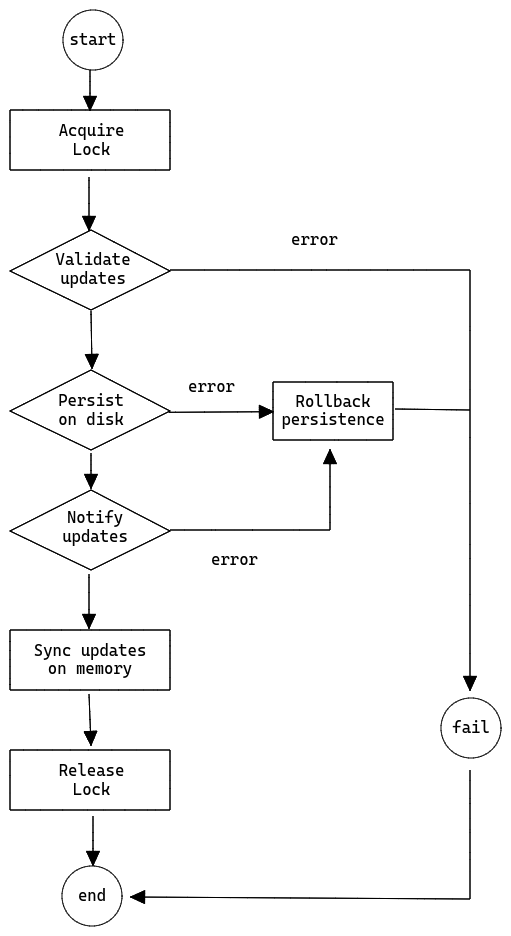
\includegraphics[width=0.6\linewidth]{draws/save.png}
    \caption{Diagrama de flujo para la función \textbf{save}.}
\end{figure}

\section{Almacenamiento en Memoria vs Disco}

Para la solución inicialmente fue considerada cargar la configuración del servidor DNS a una base de datos. Dicha solución fue desechada en favor de almacenarla en memoria. La principal desventaja de esto es tener que implementar algunos mecanismos de validación que pueden ser declarados de forma relativamente sencilla con SQL. Pero trae varias ventajas consigo, la primera y más importante es no tener dos fuentes de verdad (base de datos de la API y base de datos del servidor DNS), así cada vez que se inicie la API se garantiza que la información que sirve está sincronizada con la configuración del servidor DNS, el cual en última instancia es quien debe tener la información precisa pues es quien provee el servicio DNS.

Además, se pude obtener menores valores de latencia, dado que el acceso a valores aleatorios en memoria es mucho mas rápido que en disco (HDD o SSD)[\cite{jacobs2009pathologies}]. Además, el uso de un sistema gestor de base de datos requiere de mayores recursos de cómputo, y estamos hablando de un escenario donde se está manejando un volumen de información aceptable para ser ubicado en memoria.

\section{BIND 9}

Con el objetivo de llevar a cabo la experimentación en la implementación de una API para los servidores DNS de código abierto, se tomó como software representativo BIND 9.

\subsection{Sistema de Almacenamiento}
BIND usa como sistema de almacenamiento para el servidor DNS archivos de texto plano. En estos archivos se almacena tanto la configuración del servidor autoritario o secundario, como los archivos de zona con sus registros. En la imagen de Docker de BIND basada en Ubuntu\footnote{\url{https://hub.docker.com/r/ubuntu/bind9}} se pueden encontrar los archivos de configuración y de zona en los directorios \verb+/etc/bind+ y \verb+/var/lib/bind+ respectivamente.

\begin{lstlisting}[frame=single, numbers=none, caption=Contenido del directorio \textbf{/etc/bind}.]
$ ls /etc/bind
bind.keys  db.0  db.127  db.255  db.empty  db.local  named.conf
named.conf.default-zones  named.conf.local  named.conf.options
rndc.key  zones.rfc1918
\end{lstlisting}

El fichero principal de configuración para BIND es \verb+named.conf+, desde él se importan con la directiva \verb+include+ los demás ficheros de configuración (\verb+named.conf.*+) que se encuentran en el directorio. Así la configuración puede ser dividida en diferentes archivos, facilitando su mantenibilidad y legibilidad.

El archivo \verb+named.conf.local+ tiene las opciones globales que son usadas al iniciar el servicio. Estas son ubicadas entre llaves en el cuerpo de la declaración \verb+options+. La gramática esta disponible online en el manual de administrador para BIND\footnote{\url{https://bind9.readthedocs.io/en/v9_18_8/reference.html\#namedconf-statement-options}}. En este se manejan los aspectos fundamentales de DNS, \textit{caching}, logging a través de \verb+dnstap+, así como la configuración relacionada a DNSSEC. En este espacio también son definidas las listas de control de acceso (ACL, en inglés), que permiten restringir el acceso al servidor basado en la dirección IP del host que hace la petición. BIND dispone de gran granularidad al poder definir un ACL para cada uno de diferentes tipos de consultas que acepta el servidor.

El fichero \verb+named.conf.local+ contiene la configuración local para el servidor DNS y es donde se declaran las zonas que este va a manejar. En este también se puede hacer uso de la directiva \verb+include+, para importar otros ficheros que declaran zonas usualmente, como es el caso de \verb+zones.rfc1918+.

Una zona es definida con un nombre, una clase (por defecto \verb+IN+, por \verb+Internet+) y un cuerpo que contiene un conjunto de opciones para la zona. Dentro de estas opciones es requerido definir su tipo con la palabra clave \verb+type+. Cada tipo tiene una gramática distinta de acuerdo a las opciones que admite.

La zona dentro de sus opciones permiten definir diferentes ACL, similar a las opciones globales. Cada zona puede tener su política para manejar actualizaciones en tiempo de ejecución. Específicamente, la opción \verb+allow-update+ maneja mediante una ACL quien pude actualizar registros en una zona. De igual forma, \verb+update-policy+ permite controlar quien modifica la zona basada en la identidad del solicitante, la identidad es determinada por la clave que firmó el pedido, usando TSIG o SIG(0). Estos dos mecanismos para controlar el acceso se definen de forma excluyente y el segundo solo puede ser usado en zonas de tipo primario (\verb+primary+ o \verb+master+).

Los otros ficheros ubicados en \verb+/etc/bind+, son \verb+bind.keys+ y los \verb+db.*+. El primero tiene como objetivo sobreescribir las claves públicas (\textit{trust anchors}) que usa BIND para DNSSEC. Los segundos son empleados para indicar la zona del host y la interfaces de \textit{loopback} y \textit{broadcast}. Estos son cargados directamente por \verb+named.conf.default-zones+.

\begin{lstlisting}[frame=single, numbers=none, caption=Contenido del fichero \textbf{named.conf.default-zones}]
$ cat /etc/bind/named.conf.default-zones
// prime the server with knowledge of the root servers
zone "." {
    type hint;
    file "/usr/share/dns/root.hints";
};

// be authoritative for the localhost forward and reverse zones,
// and for broadcast zones as per RFC 1912

zone "localhost" {
    type master;
    file "/etc/bind/db.local";
};

zone "127.in-addr.arpa" {
    type master;
    file "/etc/bind/db.127";
};

zone "0.in-addr.arpa" {
    type master;
    file "/etc/bind/db.0";
};

zone "255.in-addr.arpa" {
    type master;
    file "/etc/bind/db.255";
};
\end{lstlisting}

\subsubsection{Lectura de la Configuración DNS}

Con el fin de implementar la función \verb+load+ sobre el sistema de almacenamiento de BIND se hace necesario parsear estos archivos de texto plano. Se requiere de un parser para los archivos que contienen registros y otro para los archivos de configuración, específicamente \verb+named.conf.local+, que es el que usualmente contiene las zonas añadidas por los administradores del servidor.

El proceso de \textit{parsing} permite estructurar la información en texto plano tanto al leerla como escribirla a disco. La gramática para los archivos de configuración está completamente definida en la documentación de BIND y está sujeta a los cambios que introduzca ISC en el software. En el caso de los archivos de registros no es tan sencillo, se rigen por DNS y recordar que este es un sistema en constante cambio, son añadidos nuevos tipos de registros y por tanto es una gramática que puede cambiar en el tiempo. Definirla sobre los tipos más comunes y dejar como alternativa su extensibilidad es la opción más factible en este proyecto.

\subsubsection{Escritura de la Configuración DNS}

La información resultante del proceso de \textit{parsing} puede ser modificada y escrita a disco sin inconvenientes. Así pueden ser modificado los archivos de configuración del servidor DNS de forma directa sin afectar su funcionamiento. Este proceso puede resumirse en tomar la estructura de datos resultante del \textit{parsing}, llevarla a una cadena de texto, similar a la que tuvo como origen y escribir dicha cadena al fichero de configuración.

Como indica la función \verb+save+, es necesario mantener actualizada la copia de la configuración en memoria, esto evita tener que \textit{parsear} el archivo de configuración en modificaciones posteriores. Así se realiza el \textit{parsing} una sola vez al iniciar el sistema, posteriormente solo las escrituras de la estructura de datos al archivo de configuración correspondiente.

\subsection{Comunicación con el servidor DNS}

Cuando BIND sufre cambios en los ficheros de configuración estos no son detectados y reflejados en tiempo de ejecución. Debe reiniciarse el servicio o notificarlo de que ha ocurrido una actualización. La alternativa mas eficiente es la segunda y \verb+rndc+ es la herramienta recomendada para este proceso.

\verb+rndc+ se comunica con el servidor de nombres a través de una conexión TCP, enviando comandos con una firma digital. La versión actual utiliza como algoritmos de autenticación HMAC-MD5 (por compatibilidad), HMAC-SHA1, HMAC-SHA224, HMAC-SHA256 (por defecto), HMAC-SHA384, y HMAC-SHA512. Estos utilizan una clave secreta compartida en cada lado de la conexión, lo cual provee de autenticación de tipo TSIG para la petición del comando y la respuesta del servidor. \verb+rndc+ utiliza una archivo de configuración para determinar cómo conectarse al servidor y el algoritmo y llave a emplear en la autenticación.
